
\begin{figure*}[t]
  \centering
(a)
\vtop{
\vskip-2ex
\hbox{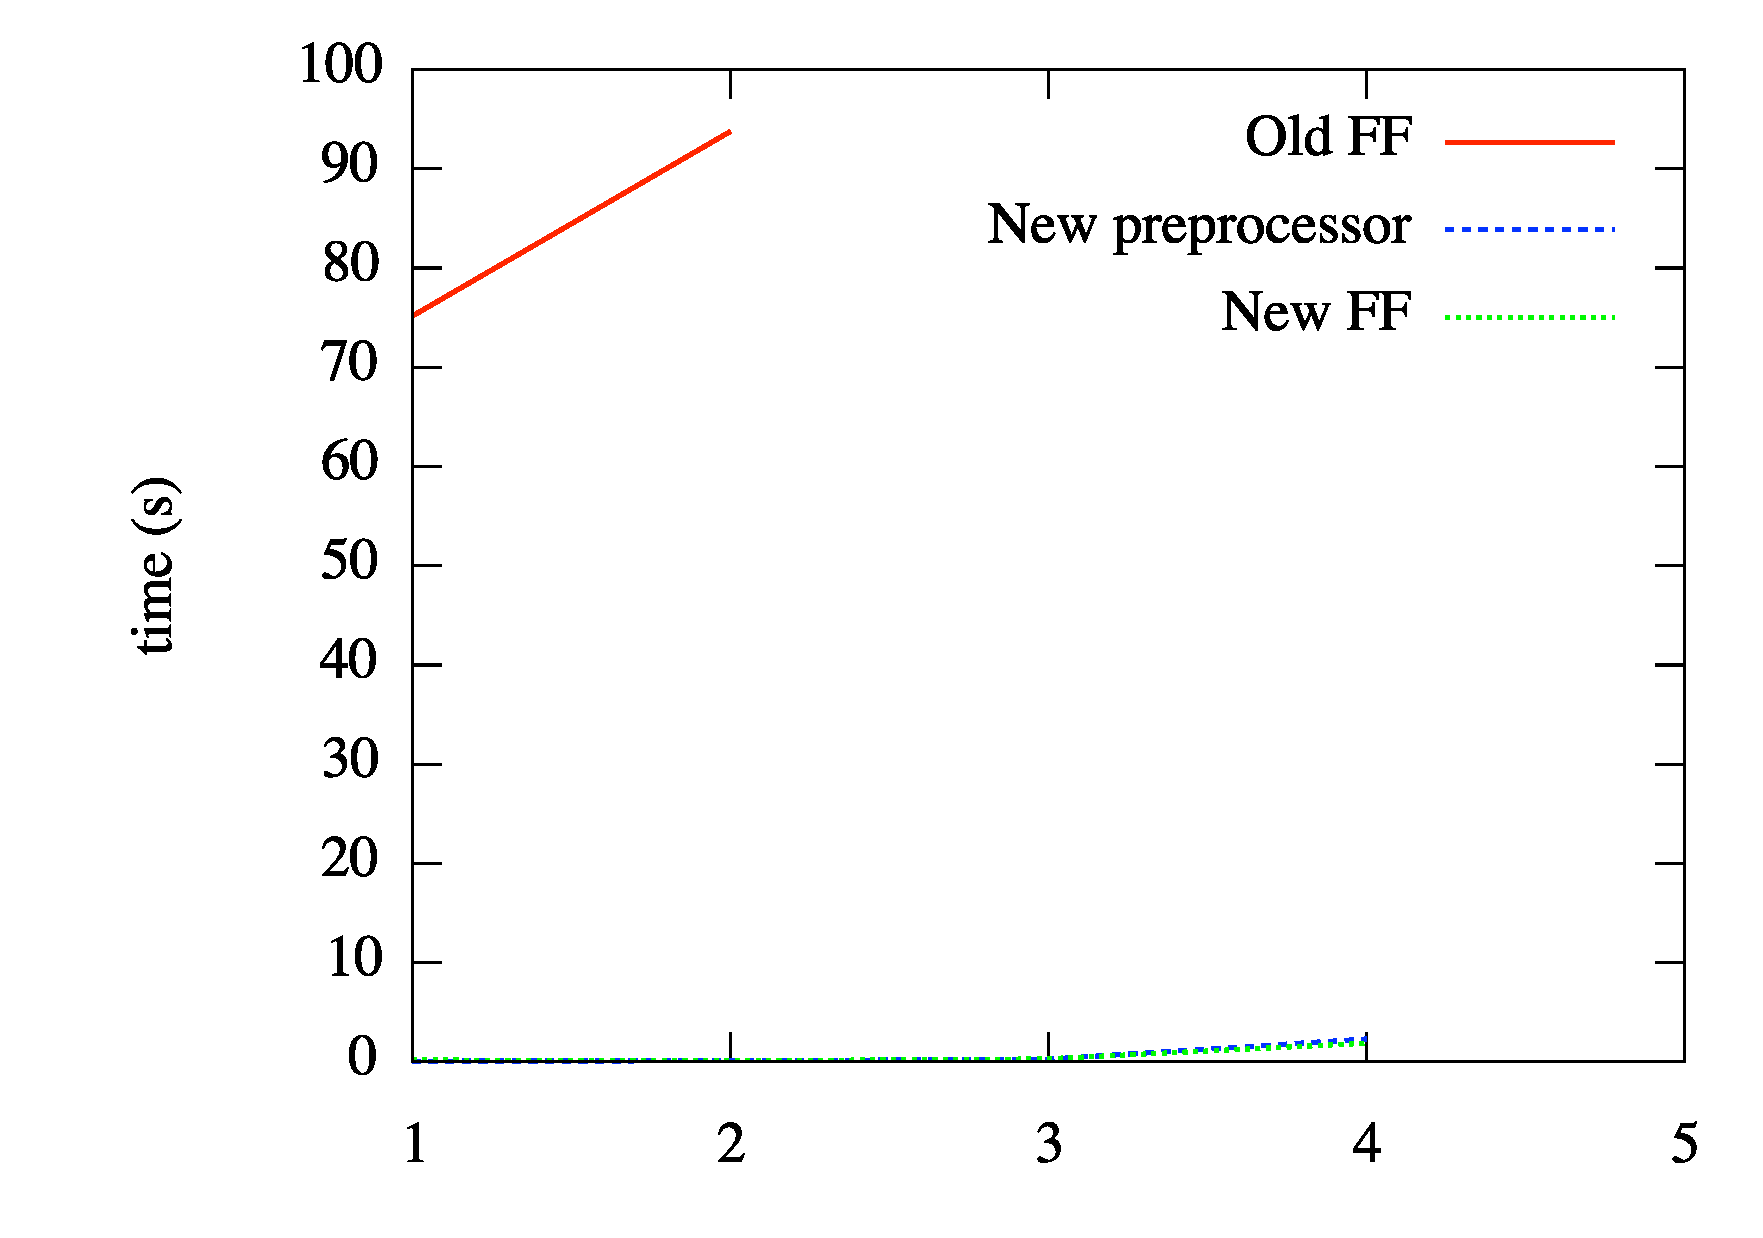
\includegraphics[width=0.8\columnwidth]{pics/xtag-k2-dist0}}
}
$\qquad\qquad$
(b)
\vtop{
\vskip-2ex
\hbox{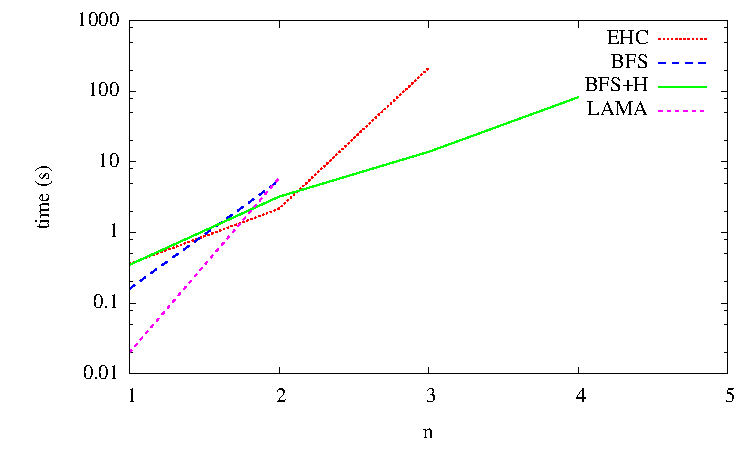
\includegraphics[width=0.8\columnwidth]{pics/xtag-k2-dist2}}
}
\vspace{-0.5cm}
\caption{Runtimes for $d=0$ (a) and $d=2$ (b).}
  \label{fig:runtimes}
\vspace{-0.5cm}
\end{figure*}


\section{Experiments} 
\label{sec:experiments}

To evaluate the effect of our changes on the efficiency of the planner
on practical inputs, we ran a series of experiments using the XTAG
Grammar \cite{xtag01:_tr}, a large-scale tree-adjoining grammar of
English, from which we selected all lexicon entries for seven words we
used in the experiments. We set up inputs to generate sentences of the
form ``$S_1$ and $S_2$ and \ldots and $S_n$'', i.e.\ a conjunction of
$n$ sentences. Each sentence $S_i$ is of the form ``X admires Y''. X
and Y are unique referring expressions, such as ``the rich
businessman''. For each experiment, we have a parameter $d$ that
specifies how many adjectives are needed to distinguish the referent
uniquely -- in particular, $d=0$ means we can say ``the businessman'',
and $d=2$ means we must say ``the rich sad businessman''.
% JOERG: ``new encoding'' gibt's ja gar nicht mehr als unterscheidung
%
%We translate
%these generation problems into planning problems with the new encoding
%as shown in Fig.~\ref{fig:white-rabbit-as-planning}.

%\begin{figure}[t]
%  \centering
%  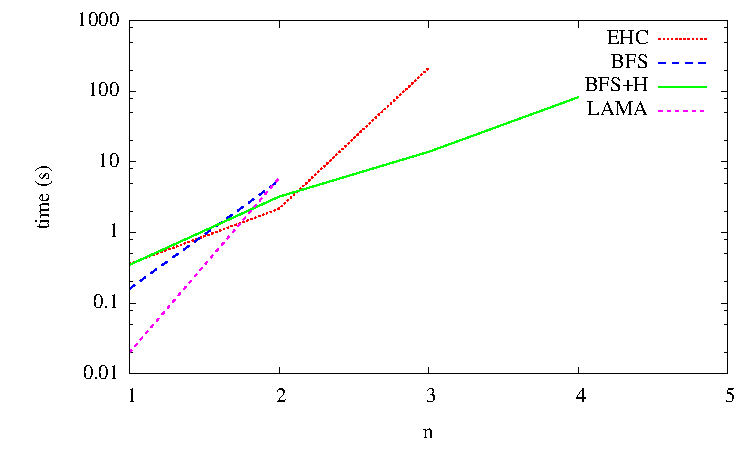
\includegraphics[width=\columnwidth]{pics/xtag-k2-dist2}
%  \caption{Runtimes for $d=2$.}
%  \label{fig:runtimes-k2-dist2}
%\end{figure}


Consider first the results for $d=0$, shown in Fig.~\ref{fig:runtimes}
(a); the lines end where the planner exceeded its five-minute timeout.
``Old FF'' in the figure is original FF, ``New preprocessor'' applies
only our fixes to FF's preprocess, ``New FF'' applies all fixes.
% The other two lines represent FF with the improved preprocessor,
%using the standard enforced hillclimbing strategy and the best-first
%search with helpful actions (``New FF'') respectively.  
Just the preprocessor fixes lead to a speed-up of at least $3$ orders
of magnitude, leading to practically useful runtime -- for instance,
the 24-word sentence at $n=4$ is generated in under two seconds. Note
that, by contrast, the search configuration does not make much of a
difference here. This changes in our next experiment.

Results for $d=2$ are shown in Fig.~\ref{fig:runtimes} (b).  Here the
old FF preprocessor crashed with a segmentation fault even at
$n=1$. Best-first search with helpful actions is clearly the
best-performing search strategy here.  It takes about 14 seconds for
$n=3$, but this sentence is already quite long at 29 words, and EHC
takes 3.5 minutes on the same input.  Best-first search without
helpful actions timed out at $n=3$, illustrating the importance of
that heuristic.

The relative behavior of the different search methods is not uniform
in our domain, which exhibits a huge amount of structural variance due
to the many different forms that the input grammar may take. We are
far from an exhaustive exploration of all the possible parameter
settings. For instance, with particular inputs (no distractors), EHC
can be more effective than best-first search.

%Suffice it to say that, in particular encoding variants and
%with particular grammars (e.g.\ grammars not featuring any
%distractors), in stark contrast to Fig.~\ref{fig:runtimes} (b) EHC is
%much more effective than best-first search.

%While this brings the overall planner runtimes into a range where FF
%can now be useful in practical NLG applications, it is important to
%note that it still has serious limitations.  The best-first search
%timed out for any $n>4$ in either experiment.  While many NLG
%applications can get by with shorter sentences, improving the search
%on our domain is still an open question for the future.  Even within
%our domain, the relative quality of EHC and BFS+H depended on the
%exact generation problem instance: While BFS+H outperformed EHC at
%$d=2$, EHC was actually slightly faster at $d=0$ because the absence
%of distractors meant there was not much room for the characteristic
%underestimation of the relaxed plan evaluation discussed above.  This
%means that sentence generation remains as a varied and challenging
%domain for planning.



%%% Local Variables: 
%%% mode: latex
%%% TeX-master: "main"
%%% End: 
